\documentclass[a4paper,11pt]{article}
\usepackage[utf8]{inputenc}
\usepackage[T1]{fontenc}
\usepackage[english]{babel}
\usepackage{tikz}
\usetikzlibrary{arrows.meta, positioning, shapes, backgrounds}
\usepackage{adjustbox}
\usepackage{geometry}
\geometry{margin=1.5cm}

\pagestyle{empty}

\begin{document}

% =====================
% GLOBAL TITLE
% =====================
\begin{center}
  \Large \textbf{Simplified Microservices Architecture -- DeepSeek}
\end{center}
\vspace{0.5cm}

% =====================
% GLOBAL DIAGRAM
% =====================
\begin{adjustbox}{max width=\textwidth, center}
\begin{tikzpicture}[
    component/.style={rectangle, draw=black, rounded corners, minimum width=2.6cm, minimum height=1cm, align=center, font=\footnotesize, fill=blue!10},
    infra/.style={rectangle, draw=black, minimum width=2.6cm, minimum height=1cm, align=center, font=\footnotesize, fill=gray!15},
    actor/.style={ellipse, draw=black, minimum width=2cm, minimum height=0.8cm, align=center, font=\footnotesize, fill=green!15},
    arrow/.style={-Latex, thick}
]

% ==== ACTORS ====
\node[actor] (web) {Web Client};
\node[actor, right=2cm of web] (mobile) {Mobile Client};

% ==== API Gateway ====
\node[component, below=1.8cm of $(web)!0.5!(mobile)$] (gateway) {API Gateway};

% ==== CORE SERVICES ====
\node[component, below=2cm of gateway] (inference) {Inference Service};
\node[component, left=3.2cm of inference] (user) {User Service};
\node[component, right=3.2cm of inference] (rag) {RAG Service};

% ==== SUPPORT ====
\node[component, below=2cm of inference, fill=orange!15] (monitor) {Monitoring \& Logs};

% ==== INFRASTRUCTURE ====
\node[infra, below=1.5cm of user] (db) {Database};
\node[infra, below=1cm of inference] (vector) {Vector Store};
\node[infra, below=1.5cm of rag] (storage) {File Storage};

% ==== CONNECTIONS ====
\draw[arrow] (web) -- (gateway);
\draw[arrow] (mobile) -- (gateway);

\draw[arrow] (gateway) -- (user);
\draw[arrow] (gateway) -- (inference);
\draw[arrow] (gateway) -- (rag);

\draw[arrow] (user) -- (db);
\draw[arrow] (inference) -- (vector);
\draw[arrow] (rag) -- (storage);

\draw[arrow, dashed] (user) -- (monitor);
\draw[arrow, dashed] (inference) -- (monitor);
\draw[arrow, dashed] (rag) -- (monitor);

% ==== LEGEND ====
\node[draw, fill=white, rounded corners, below=1.5cm of monitor, align=left, font=\scriptsize] (legend) {
  \textbf{Legend:}\\
  \begin{tabular}{@{}l@{\hspace{0.6em}}l@{}}
    \tikz\draw[fill=green!15, draw=black] (0,0) ellipse (0.35 and 0.25); & Client \\
    \tikz\draw[fill=blue!10, draw=black, rounded corners] (0,0) rectangle (0.45,0.3); & Microservice \\
    \tikz\draw[fill=orange!15, draw=black, rounded corners] (0,0) rectangle (0.45,0.3); & Support \\
    \tikz\draw[fill=gray!15, draw=black] (0,0) rectangle (0.45,0.3); & Infrastructure \\
    \tikz{\draw[arrow] (0,0) -- (0.5,0);} & Communication \\
    \tikz{\draw[arrow, dashed] (0,0) -- (0.5,0);} & Monitoring
  \end{tabular}
};

\end{tikzpicture}
\end{adjustbox}
\section{Enhanced Microservices Architectures - DeepSeek}
\begin{adjustbox}{max width=\textwidth, center}
\begin{tikzpicture}[
    component/.style={rectangle, draw=black, rounded corners, minimum width=2.6cm, minimum height=1cm, align=center, font=\footnotesize, fill=blue!10},
    infra/.style={rectangle, draw=black, minimum width=2.6cm, minimum height=1cm, align=center, font=\footnotesize, fill=gray!15},
    actor/.style={ellipse, draw=black, minimum width=2cm, minimum height=0.8cm, align=center, font=\footnotesize, fill=green!15},
    arrow/.style={-Latex, thick},
    dashedarrow/.style={-Latex, dashed, thick, gray}
]

% ==== ACTORS ====
\node[actor] (web) {Web Client};
\node[actor, right=2cm of web] (mobile) {Mobile Client};

% ==== API Gateway ====
\node[component, below=1.8cm of $(web)!0.5!(mobile)$] (gateway) {API Gateway};

% ==== AUTH SERVICE ====
\node[component, left=2.5cm of gateway, fill=orange!15] (auth) {Auth Service};

% ==== CORE SERVICES ====
\node[component, below=2cm of gateway] (inference) {Inference Service};
\node[component, left=3.2cm of inference] (user) {User Service};
\node[component, right=3.2cm of inference] (rag) {RAG Service};

% ==== NEW: MODEL MANAGEMENT SERVICE ====
\node[component, below=3cm of inference, fill=blue!15] (model) {Model Management Service};

% ==== SUPPORT ====
\node[component, below=3cm of model, fill=orange!15] (monitor) {Monitoring \& Logs};

% ==== INFRASTRUCTURE ====
\node[infra, below=1.5cm of user] (db) {Database};
\node[infra, below=1cm of inference] (vector) {Vector Store};
\node[infra, below=1.5cm of rag] (storage) {File Storage};

% ==== NEW: MESSAGE BROKER ====
\node[infra, below=1.5cm of model, fill=gray!20] (broker) {Message Broker};

% ==== CONNECTIONS ====

% --- Clients to Gateway ---
\draw[arrow] (web) -- (gateway);
\draw[arrow] (mobile) -- (gateway);

% --- Gateway to Services ---
\draw[arrow] (gateway) -- (user);
\draw[arrow] (gateway) -- (inference);
\draw[arrow] (gateway) -- (rag);

% --- Gateway to Auth ---
\draw[dashedarrow] (gateway) -- (auth);

% --- Core Services to Infra ---
\draw[arrow] (user) -- (db);
\draw[arrow] (inference) -- (vector);
\draw[arrow] (rag) -- (storage);

% --- Model Management Links ---
\draw[arrow] (inference) -- (model);
\draw[arrow] (model) -- (broker);

% --- Message Broker Links ---
\draw[arrow, dashed] (broker) -- (user);
\draw[arrow, dashed] (broker) -- (inference);
\draw[arrow, dashed] (broker) -- (rag);

% --- Monitoring ---
\foreach \s in {user, inference, rag, model} {
    \draw[dashedarrow] (\s) -- (monitor);
}

% ==== LEGEND ====
\node[draw, fill=white, rounded corners, below=1.5cm of broker, align=left, font=\scriptsize] (legend) {
  \textbf{Legend:}\\
  \begin{tabular}{@{}l@{\hspace{0.6em}}l@{}}
    \tikz\draw[fill=green!15, draw=black] (0,0) ellipse (0.35 and 0.25); & Client \\
    \tikz\draw[fill=blue!10, draw=black, rounded corners] (0,0) rectangle (0.45,0.3); & Microservice \\
    \tikz\draw[fill=orange!15, draw=black, rounded corners] (0,0) rectangle (0.45,0.3); & Security/Support \\
    \tikz\draw[fill=gray!15, draw=black] (0,0) rectangle (0.45,0.3); & Infrastructure \\
    \tikz{\draw[arrow] (0,0) -- (0.5,0);} & Main Communication \\
    \tikz{\draw[dashedarrow] (0,0) -- (0.5,0);} & Async/Monitoring Link
  \end{tabular}
};

\end{tikzpicture}
\end{adjustbox}

% =====================
% API GATEWAY ANALYSIS
% =====================
\newpage
\section{API Gateway Analysis}

\subsection*{Role and Definition}
The API Gateway acts as a single entry point for clients.  
It centralizes access to microservices and ensures critical functions such as routing, security, and data aggregation.

\subsection*{Main Responsibilities}
\begin{itemize}
    \item Request routing to microservices.
    \item Aggregation of responses from multiple services.
    \item Authentication and authorization (OAuth2, JWT).
    \item Protocol transformation (REST, gRPC, WebSocket).
    \item Metrics and logs collection for monitoring.
    \item Rate limiting and throttling.
\end{itemize}

\subsection*{Advantages}
\begin{itemize}
    \item Simplifies client access with a single entry point.
    \item Centralizes security and global policies.
    \item Supports response aggregation and improves performance.
    \item Facilitates scalability and modularity.
\end{itemize}

\subsection*{Limitations}
\begin{itemize}
    \item Risk of \textbf{Single Point of Failure}.
    \item Additional latency.
    \item Complexity in configuration and maintenance.
\end{itemize}

% =====================
% UML DIAGRAM - API GATEWAY
% =====================
\begin{center}
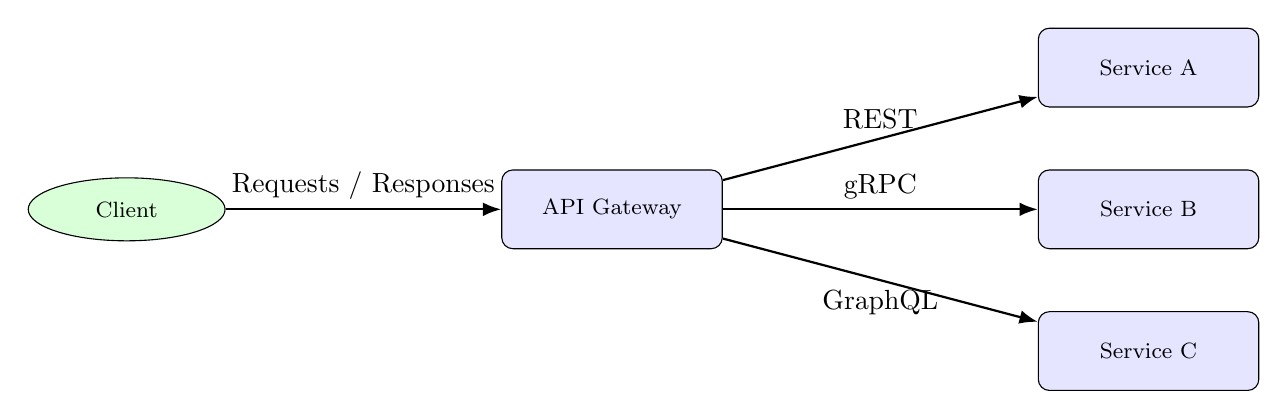
\begin{tikzpicture}[
    component/.style={rectangle, draw=black, rounded corners, minimum width=2.8cm, minimum height=1cm, align=center, font=\footnotesize, fill=blue!10},
    actor/.style={ellipse, draw=black, minimum width=2.5cm, minimum height=0.8cm, align=center, font=\footnotesize, fill=green!15},
    arrow/.style={-Latex, thick}
]

% ==== Client ====
\node[actor] (client) {Client};

% ==== API Gateway ====
\node[component, right=3.5cm of client] (apigw) {API Gateway};

% ==== Microservices ====
\node[component, right=4cm of apigw, yshift=1.8cm] (serviceA) {Service A};
\node[component, right=4cm of apigw] (serviceB) {Service B};
\node[component, right=4cm of apigw, yshift=-1.8cm] (serviceC) {Service C};

% ==== Relations ====
\draw[arrow] (client) -- (apigw) node[midway, above]{Requests / Responses};
\draw[arrow] (apigw) -- (serviceA) node[midway, above]{REST};
\draw[arrow] (apigw) -- (serviceB) node[midway, above]{gRPC};
\draw[arrow] (apigw) -- (serviceC) node[midway, below]{GraphQL};

\end{tikzpicture}
\end{center}

\captionof{figure}{UML diagram of the API Gateway and its interactions.}


\section{\textbf{Internal Architecture of the API Gateway}} 

\vspace{0.5cm}

\begin{center}
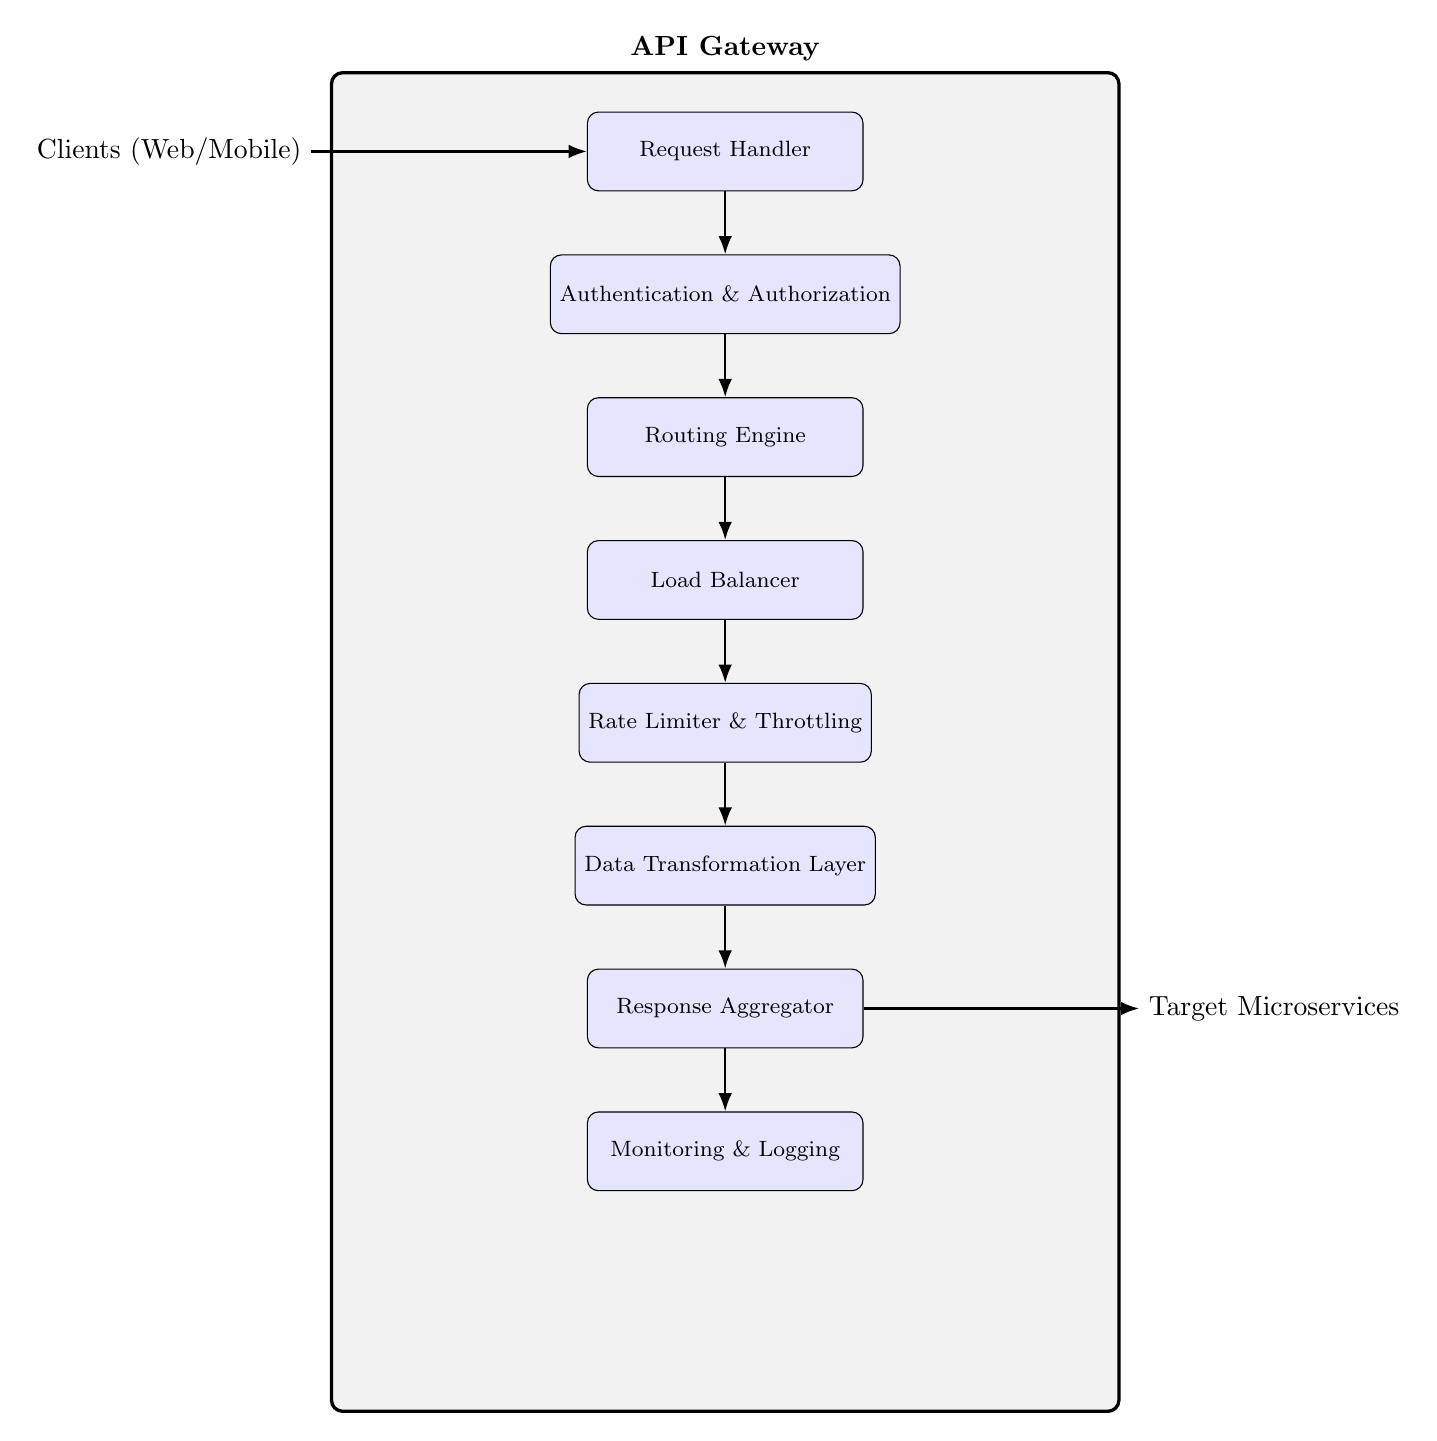
\begin{tikzpicture}[
    component/.style={rectangle, draw=black, rounded corners, minimum width=3.5cm, minimum height=1cm, align=center, font=\footnotesize, fill=blue!10},
    arrow/.style={-Latex, thick}
]

% ==== API Gateway container ====
\node[rectangle, draw=black, very thick, rounded corners, minimum width=10cm, minimum height=17cm, label={[yshift=0cm]above:\textbf{API Gateway}}, fill=gray!10] (gateway) {};

% ==== Internal components ====
\node[component, yshift=7.5cm] (reqhandler) {Request Handler};
\node[component, below=0.8cm of reqhandler] (auth) {Authentication \& Authorization};
\node[component, below=0.8cm of auth] (routing) {Routing Engine};
\node[component, below=0.8cm of routing] (loadbal) {Load Balancer};
\node[component, below=0.8cm of loadbal] (ratelimit) {Rate Limiter \& Throttling};
\node[component, below=0.8cm of ratelimit] (transform) {Data Transformation Layer};
\node[component, below=0.8cm of transform] (aggregator) {Response Aggregator};
\node[component, below=0.8cm of aggregator] (monitor) {Monitoring \& Logging};

% ==== Arrows (internal flow) ====
\draw[arrow] (reqhandler) -- (auth);
\draw[arrow] (auth) -- (routing);
\draw[arrow] (routing) -- (loadbal);
\draw[arrow] (loadbal) -- (ratelimit);
\draw[arrow] (ratelimit) -- (transform);
\draw[arrow] (transform) -- (aggregator);
\draw[arrow] (aggregator) -- (monitor);

% ==== External labels ====
\node[left=3.5cm of reqhandler] (client) {Clients (Web/Mobile)};
\draw[arrow] (client) -- (reqhandler);

\node[right=3.5cm of aggregator] (services) {Target Microservices};
\draw[arrow] (aggregator) -- (services);

\end{tikzpicture}
\end{center}

% ------------------------
% Detailed Analysis : API Gateway
% ------------------------
\section{Detailed Analysis — Internal Architecture of the API Gateway}

\subsection{Objectives and Requirements}
The API Gateway plays a central role in controlling and orchestrating client access to DeepSeek's microservices.  

\textbf{Functional Objectives}:
\begin{itemize}
  \item Provide a unified and stable entry point for all clients (Web, Mobile, Third-party APIs).
  \item Authenticate and authorize requests.
  \item Route requests to the appropriate services and aggregate responses when necessary.
  \item Perform protocol and data format transformations (REST $\leftrightarrow$ gRPC, JSON, GraphQL).
  \item Enforce policies (rate limiting, quotas, canary routing).
\end{itemize}

\textbf{Non-Functional Requirements}:
\begin{itemize}
  \item High availability (replicas, multi-zone deployment).
  \item Low latency and ability to handle traffic spikes.
  \item Observability (metrics, logs, traces).
  \item Security (TLS, validation, WAF).
  \item Easy configuration and policy enforcement.
\end{itemize}

\subsection{Internal Components — Detailed Description}
\begin{description}
  \item[Request Handler] : entry point receiving HTTP/WS requests, extracting headers, body, correlation IDs; performs syntactic validations (size, JSON schema) and applies basic protections (payload limits).
  \item[Authentication \& Authorization] : verifies JWT/OAuth2 (signature via JWKS) or opaque tokens (introspection with an Auth Service). Enforces scope/role checks (RBAC/ABAC).
  \item[Rate Limiter \& Throttling] : applies quotas per key (IP, API key, userId). Common implementations: token-bucket or leaky-bucket, atomic counters in Redis (Lua scripts) for cluster safety.
  \item[Input Validation \& Sanitization] : schema validation, header sanitization, normalization (unicode, trim), injection protection.
  \item[Routing Engine / Service Discovery] : maps requests (path, host, header) to target services. Integrates discovery (Consul / Kubernetes API) and routing rules (versions, canary, A/B testing).
  \item[Load Balancer / Upstream Manager] : selects upstream instance (RoundRobin, least-connections, weighted), manages persistent connections (keep-alive), handles timeouts.
  \item[Circuit Breaker \& Retry Policy] : protects against degraded upstreams. Key parameters: failure threshold, time window, reset timeout, exponential backoff retry logic.
  \item[Protocol / Data Transformation] : converts REST $\leftrightarrow$ gRPC, shapes JSON, maps schemas, enriches responses, strips sensitive fields before sending.
  \item[Response Aggregator / Composer] : orchestrates parallel service calls, merges results, supports partial responses and fallback strategies.
  \item[Monitoring \& Logging] : exports structured logs, traces, and metrics (Prometheus, OpenTelemetry) for observability.
\end{description}

% =====================
% IMPROVEMENTS
% =====================
\section{Proposed Improvements for the API Gateway}

The \textbf{DeepSeek API Gateway} can be enhanced to improve security, performance, and governance.  
Key additions include:  

\begin{itemize}
  \item \textbf{Security:} WAF (Web Application Firewall), mTLS support, OAuth2 validation.
  \item \textbf{Performance:} distributed caching, intelligent load balancing, circuit breaker and retry logic.
  \item \textbf{Observability:} distributed tracing (OpenTelemetry), advanced monitoring, Prometheus metrics.
  \item \textbf{Flexibility:} multi-protocol support (REST, gRPC, GraphQL), data aggregation and advanced transformation.
  \item \textbf{Governance:} API schema validation (OpenAPI/JSON Schema), quotas, versioning, and service discovery.
\end{itemize}

\vspace{0.5cm}

\begin{center}
\Large \textbf{Enhanced Internal Architecture of the API Gateway}
\end{center}
\vspace{0.5cm}

\begin{adjustbox}{max width=\textwidth, center}
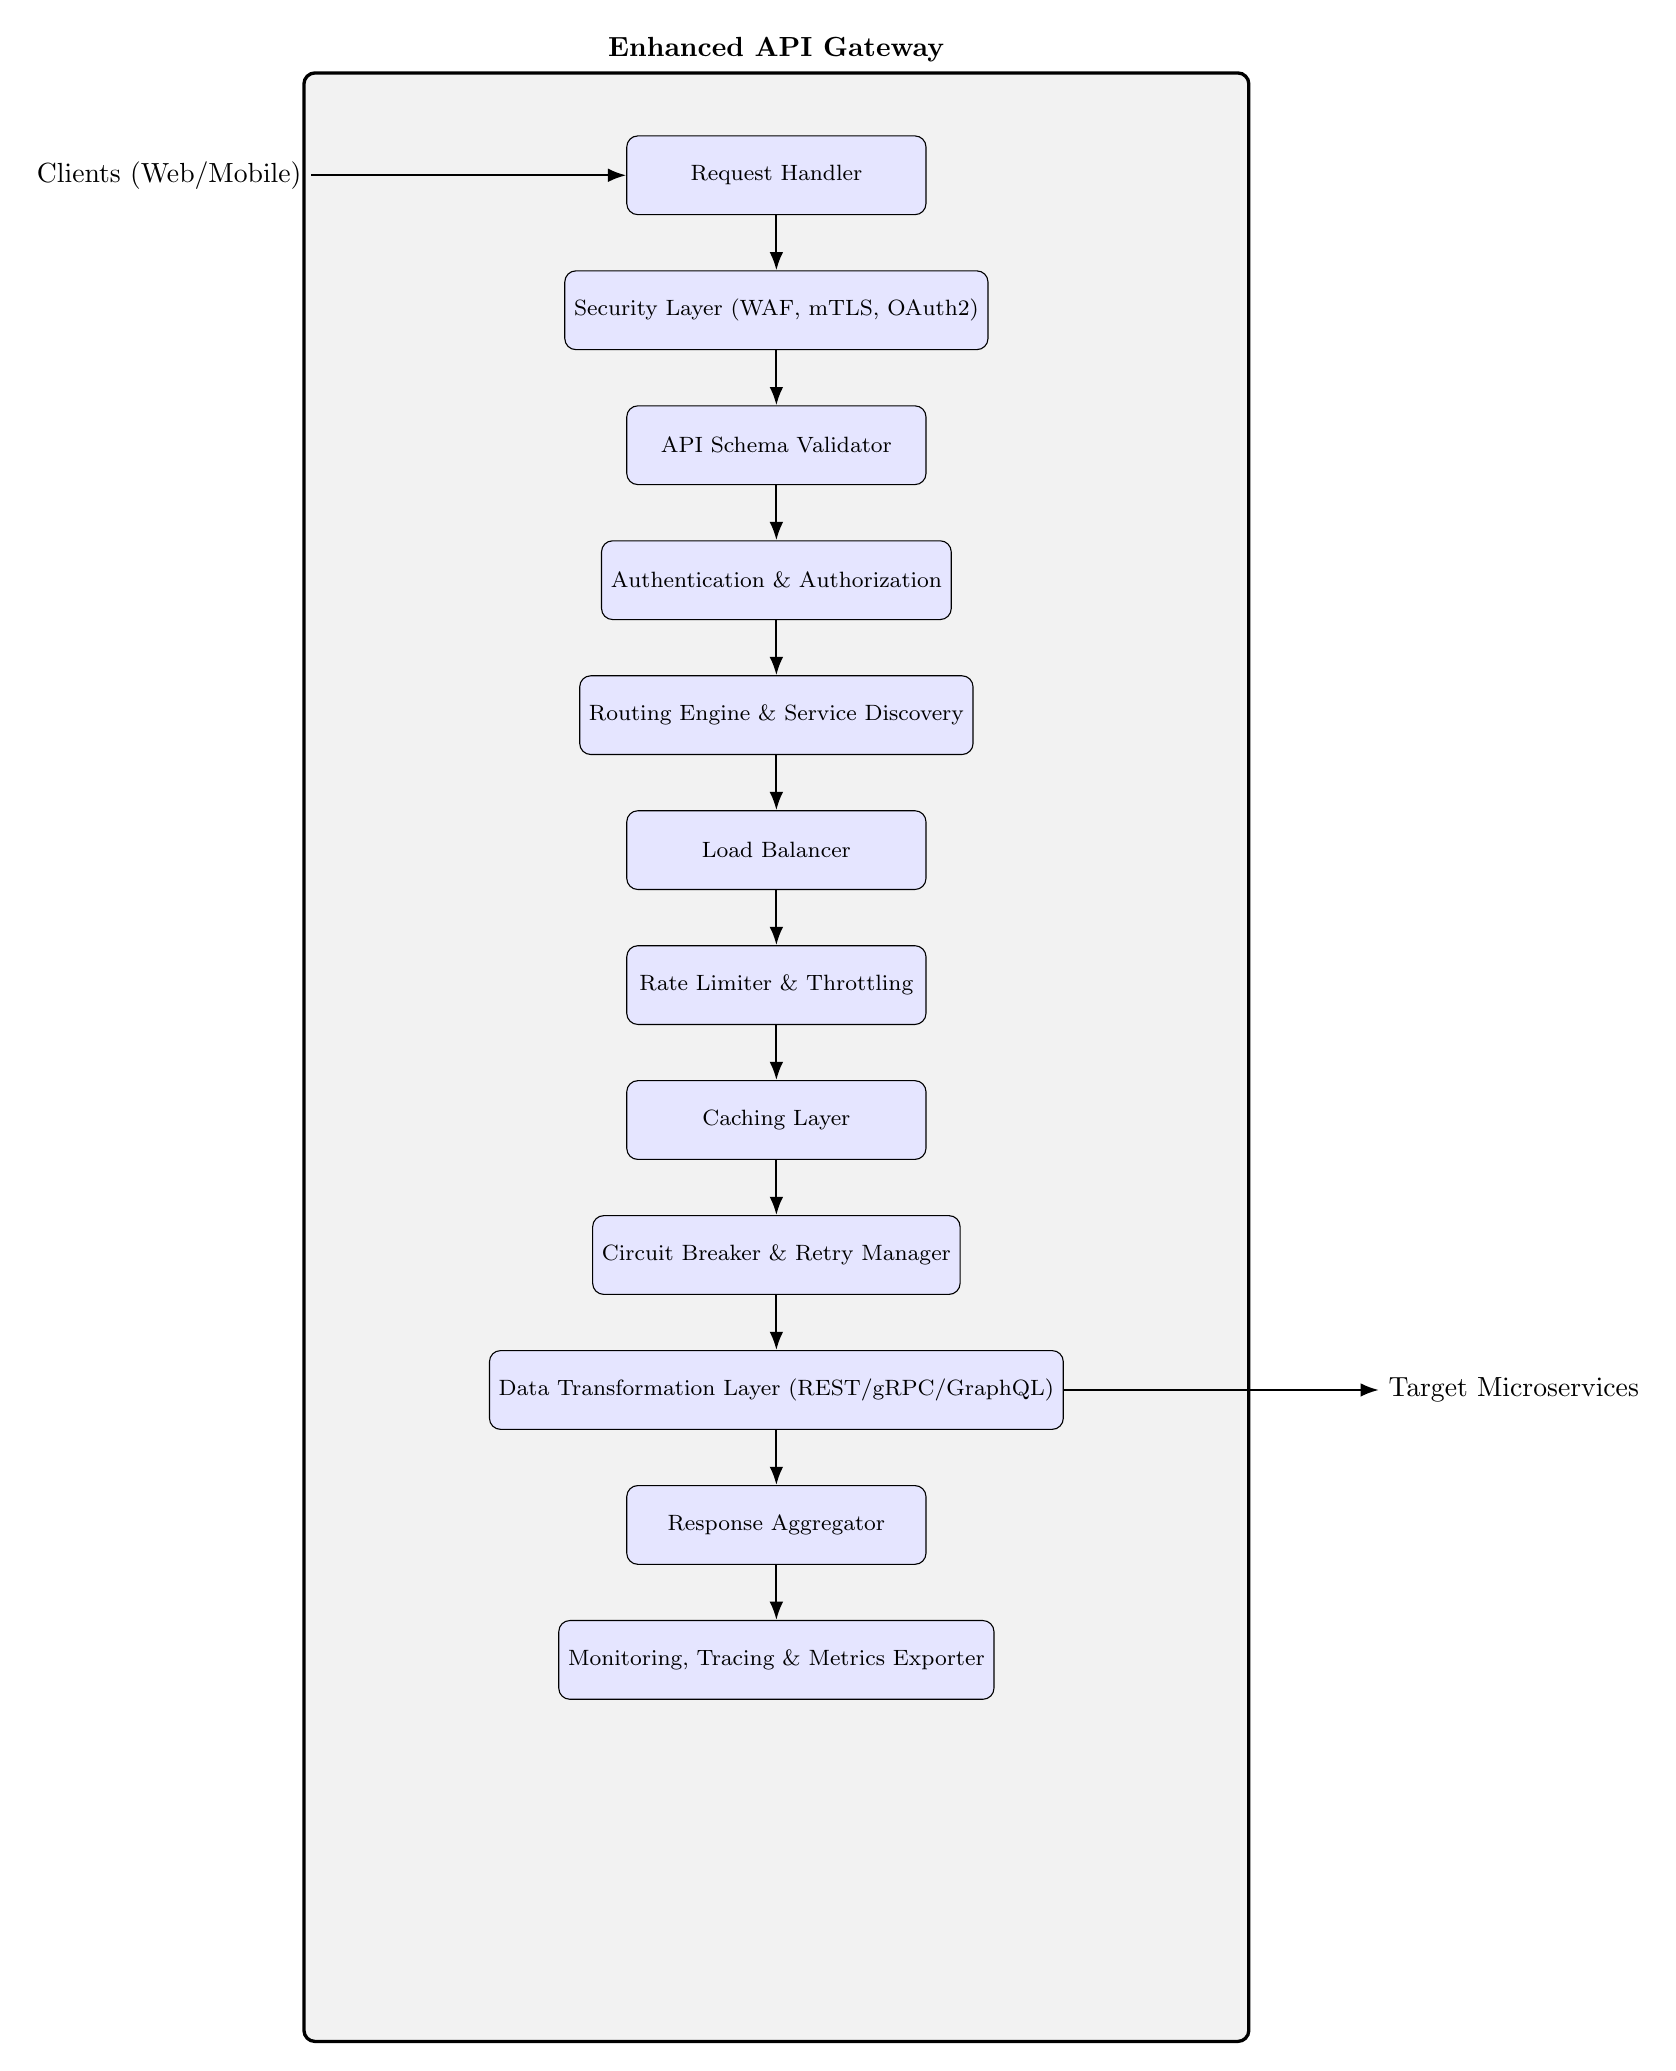
\begin{tikzpicture}[
    component/.style={rectangle, draw=black, rounded corners, minimum width=3.8cm, minimum height=1cm, align=center, font=\footnotesize, fill=blue!10},
    arrow/.style={-Latex, thick}
]

% ==== API Gateway container ====
\node[rectangle, draw=black, very thick, rounded corners, minimum width=12cm, minimum height=25cm, label={[yshift=0cm]above:\textbf{Enhanced API Gateway}}, fill=gray!10] (gateway) {};

% ==== Internal components ====
\node[component, yshift=11.2cm] (reqhandler) {Request Handler};
\node[component, below=0.7cm of reqhandler] (waf) {Security Layer (WAF, mTLS, OAuth2)};
\node[component, below=0.7cm of waf] (apivalid) {API Schema Validator};
\node[component, below=0.7cm of apivalid] (auth) {Authentication \& Authorization};
\node[component, below=0.7cm of auth] (routing) {Routing Engine \& Service Discovery};
\node[component, below=0.7cm of routing] (loadbal) {Load Balancer};
\node[component, below=0.7cm of loadbal] (ratelimit) {Rate Limiter \& Throttling};
\node[component, below=0.7cm of ratelimit] (cache) {Caching Layer};
\node[component, below=0.7cm of cache] (circuit) {Circuit Breaker \& Retry Manager};
\node[component, below=0.7cm of circuit] (transform) {Data Transformation Layer (REST/gRPC/GraphQL)};
\node[component, below=0.7cm of transform] (aggregator) {Response Aggregator};
\node[component, below=0.7cm of aggregator] (monitor) {Monitoring, Tracing \& Metrics Exporter};

% ==== Arrows (internal flow) ====
\draw[arrow] (reqhandler) -- (waf);
\draw[arrow] (waf) -- (apivalid);
\draw[arrow] (apivalid) -- (auth);
\draw[arrow] (auth) -- (routing);
\draw[arrow] (routing) -- (loadbal);
\draw[arrow] (loadbal) -- (ratelimit);
\draw[arrow] (ratelimit) -- (cache);
\draw[arrow] (cache) -- (circuit);
\draw[arrow] (circuit) -- (transform);
\draw[arrow] (transform) -- (aggregator);
\draw[arrow] (aggregator) -- (monitor);

% ==== External labels ====
\node[left=4cm of reqhandler] (client) {Clients (Web/Mobile)};
\draw[arrow] (client) -- (reqhandler);

\node[right=4cm of transform] (services) {Target Microservices};
\draw[arrow] (transform) -- (services);

\end{tikzpicture}
\end{adjustbox}

\section{\textbf{Client Request Execution Scenario - DeepSeek API Gateway}} 

\vspace{0.5cm}

\section*{Step-by-Step Scenario}

\begin{enumerate}
    \item \textbf{Client Request:} Web/Mobile client sends a request (REST/GraphQL) with JWT/OAuth2 token.
    \item \textbf{Request Handler:} Validates headers, payload, and assigns correlation ID.
    \item \textbf{Security Layer:} WAF blocks malicious patterns, mTLS ensures client identity, OAuth2 token validation.
    \item \textbf{API Schema Validator:} Validates request against OpenAPI/JSON Schema.
    \item \textbf{Authentication \& Authorization:} Checks RBAC/ABAC, denies unauthorized requests.
    \item \textbf{Routing Engine \& Service Discovery:} Maps request to appropriate microservices.
    \item \textbf{Load Balancer:} Selects upstream instances, manages connections and timeouts.
    \item \textbf{Rate Limiter \& Throttling:} Applies per-user/API key quotas.
    \item \textbf{Caching Layer:} Returns cached response if available, otherwise forwards request.
    \item \textbf{Circuit Breaker \& Retry:} Protects upstream services, retries failed calls, applies fallback if needed.
    \item \textbf{Data Transformation Layer:} Converts REST $\leftrightarrow$ gRPC/GraphQL, enriches request.
    \item \textbf{Microservice Calls:} Calls User, Inference, and RAG services in parallel.
    \item \textbf{Response Aggregator:} Combines results into a unified response, handles partial failures.
    \item \textbf{Monitoring \& Metrics:} Logs request/response, updates traces and metrics.
    \item \textbf{Client Response:} Sends aggregated response back to the client securely (TLS).
\end{enumerate}

\vspace{0.5cm}
\section{Parallel Microservices Architecture in DeepSeek}
\begin{adjustbox}{max width=\textwidth, center}
\begin{tikzpicture}[
  component/.style={rectangle, draw=black, rounded corners, minimum width=3cm, minimum height=0.9cm, align=center, font=\footnotesize, fill=blue!10},
  infra/.style={rectangle, draw=black, minimum width=2.6cm, minimum height=0.9cm, align=center, font=\footnotesize, fill=gray!15},
  actor/.style={ellipse, draw=black, minimum width=2.2cm, minimum height=0.8cm, align=center, font=\footnotesize, fill=green!15},
  arrow/.style={-Latex, thick, black},
  dashedarrow/.style={-Latex, dashed, thick, gray!60},
  label/.style={font=\tiny\itshape, above, sloped}
]

% ========== COUCHE CLIENTS ==========
\node[actor] (web) {Web Client};
\node[actor, right=3cm of web] (mobile) {Mobile Client};

% ========== COUCHE RÉSEAU ==========
\node[infra, below=1.2cm of $(web)!0.5!(mobile)$] (cdn) {CDN / Edge Cache};

% ========== COUCHE API ==========
\node[component, below=1.5cm of cdn] (gateway) {API Gateway Cluster};
\node[component, left=1.8cm of gateway] (bff) {BFF (per-client)};
\node[component, left=1.8cm of bff, fill=orange!15] (auth) {Auth Service};

% ========== COUCHE SERVICES ==========
\node[component, below=1.8cm of gateway] (api) {API Orchestrator};
\node[component, left=2.2cm of api] (user) {User Service};
\node[component, right=2.2cm of api] (rag) {RAG / Retrieval};
\node[component, below=0.8cm of api] (inference) {Inference Service};

% ========== COUCHE MODÈLES ==========
\node[component, below=1.5cm of inference, fill=blue!15] (model) {Model Mgmt \& Serving};
\node[infra, left=2.2cm of model] (broker) {Message Broker (Kafka)};

% ========== COUCHE DONNÉES ==========
\node[infra, below=1.5cm of user] (db) {DB (sharded + replicas)};
\node[infra, below=1.5cm of rag] (storage) {Object Storage / FS};
\node[infra, below=1.5cm of model] (vector) {Vector DB (sharded)};

% ========== MONITORING ==========
\node[infra, right=0.8cm of storage, fill=orange!10, minimum width=2.8cm] (monitor) {Metrics \& Tracing};

% ========== CONNECTIONS PRINCIPALES ==========

% Clients vers CDN
\draw[arrow] (web) -- node[label] {HTTP/HTTPS} (cdn);
\draw[arrow] (mobile) -- node[label] {HTTP/HTTPS} (cdn);

% CDN vers Gateway
\draw[arrow] (cdn) -- node[label] {Load Balancing} (gateway);

% Gateway vers services d'API
\draw[arrow] (gateway) -- node[label] {Routing} (bff);
\draw[dashedarrow] (gateway) -- node[label, black] {Auth} (auth);

% API vers services métier
\draw[arrow] (bff) -- node[label] {API Calls} (api);
\draw[arrow] (api) -- node[label] {Data} (user);
\draw[arrow] (api) -- node[label] {Queries} (rag);
\draw[arrow] (api) -- node[label] {Inference} (inference);

% Services vers modèles
\draw[arrow] (inference) -- node[label] {Model Calls} (model);
\draw[arrow] (model) -- node[label] {Async Events} (broker);

% Broker vers services (communication asynchrone)
\draw[dashedarrow] (broker) -- node[label] {Events} (user);
\draw[dashedarrow] (broker) -- node[label] {Events} (inference);
\draw[dashedarrow] (broker) -- node[label] {Events} (rag);

% Services vers stockage
\draw[arrow] (user) -- node[label] {CRUD} (db);
\draw[arrow] (rag) -- node[label] {Vectors} (vector);
\draw[arrow] (inference) -- node[label] {Embeddings} (vector);
\draw[arrow] (rag) -- node[label] {Files} (storage);

% Monitoring
\foreach \s in {user,inference,rag,model} {
  \draw[dashedarrow] (\s) -- node[label] {Metrics} (monitor);
}

% ========== LÉGENDE ET GROUPES ==========
\begin{scope}[on background layer]
  \draw[fill=blue!5, rounded corners] 
    ($(web.north west)+(-0.3,0.5)$) rectangle 
    ($(mobile.north east)+(0.3,-1)$)
    node[above left] {\scriptsize\textbf{Clients}};
    
  \draw[fill=green!5, rounded corners] 
    ($(cdn.north west)+(-0.3,0.3)$) rectangle 
    ($(gateway.south east)+(0.3,-0.3)$)
    node[above left] {\scriptsize\textbf{API Layer}};
    
  \draw[fill=yellow!5, rounded corners] 
    ($(api.north west)+(-0.3,0.3)$) rectangle 
    ($(rag.south east)+(0.3,-1)$)
    node[above left] {\scriptsize\textbf{Business Layer}};
    
  \draw[fill=red!5, rounded corners] 
    ($(db.north west)+(-0.3,0.3)$) rectangle 
    ($(storage.south east)+(0.3,-0.3)$)
    node[above left] {\scriptsize\textbf{Data Layer}};
\end{scope}

\end{tikzpicture}
\end{adjustbox}

\vspace{0.5cm}

The illustrated architecture represents the \textbf{Parallel Microservices Architecture of DeepSeek}, designed to optimize concurrency, scalability, and fault tolerance. The main goal of this design is to process a high volume of client requests simultaneously by distributing workloads across independent and parallelized service layers.

At the top of the architecture, two types of clients—\textbf{Web Client} and \textbf{Mobile Client}—interact with the system through secure \textbf{HTTP/HTTPS} requests. These requests are first routed through a global \textbf{CDN (Content Delivery Network) / Edge Cache}, which accelerates content delivery and reduces latency by caching responses near the user.

Next, all incoming traffic is processed by the \textbf{API Gateway Cluster}, the central entry point of the system. The gateway performs load balancing, routing, and authentication by forwarding requests either to the \textbf{BFF (Backend-for-Frontend)} components—optimized for each type of client—or directly to the \textbf{Auth Service} for user validation and token verification. This ensures that every client request is efficiently authenticated before being distributed to backend services.

Once authorized, the requests reach the \textbf{API Orchestrator}, which coordinates the execution of multiple backend microservices in parallel. For example, user-related requests are sent to the \textbf{User Service}, knowledge retrieval tasks to the \textbf{RAG (Retrieval-Augmented Generation) Service}, and inference requests to the \textbf{Inference Service}. These services run concurrently, independently accessing their required resources and returning results asynchronously. The orchestrator then aggregates all partial outputs to build the final response, reducing total response time through parallel execution.

At the model layer, the \textbf{Model Management \& Serving} component handles model versioning, deployment, and serving. It communicates asynchronously with the \textbf{Message Broker (Kafka)}, which broadcasts events across services using a publish/subscribe mechanism. This enables event-driven parallel processing, allowing multiple microservices (e.g., User, Inference, and RAG) to react to the same event simultaneously, improving throughput and scalability.

The \textbf{Data Layer} includes multiple specialized storage systems operating in parallel. A \textbf{Sharded Database} handles transactional data, the \textbf{Vector Database} stores embeddings for semantic search and retrieval, and the \textbf{Object Storage} manages large unstructured files. These distributed data systems enable concurrent read and write operations, supporting the high throughput demands of parallel microservices.

To ensure system observability, all services continuously send logs, metrics, and traces to a centralized \textbf{Monitoring and Tracing} infrastructure. This allows developers and operators to track performance bottlenecks, identify latency issues, and optimize the parallel execution flow in real time.

Overall, this architecture emphasizes:
\begin{itemize}
    \item \textbf{Parallel Execution:} Requests are handled by multiple services at once, reducing total processing time.
    \item \textbf{Scalability:} Each component can scale independently based on workload intensity.
    \item \textbf{Asynchronous Communication:} Event-driven processing ensures non-blocking interactions between services.
    \item \textbf{High Availability:} Redundant components and clusters ensure fault tolerance and resilience under heavy load.
\end{itemize}

This design enables DeepSeek to efficiently manage large-scale workloads, providing rapid and reliable responses even under high concurrency, which is essential for real-time AI inference and research-intensive operations.
\section{Optimality of the Parallel Microservices Architecture}

The proposed architecture for DeepSeek aims to maximize throughput and minimize latency under high-concurrency workloads. We formalize its optimality based on parallel execution principles and queueing theory.

\subsection{Latency Reduction via Parallelism}

Let a request be decomposed into independent tasks $T_1, T_2, \dots, T_n$. In a sequential design, total latency is:
\[
L_{\text{seq}} = \sum_{i=1}^{n} T_i
\]
With parallel execution, independent tasks can run concurrently, reducing latency to:
\[
L_{\text{par}} = \max_{i} T_i + L_{\text{agg}}
\]
where $L_{\text{agg}}$ is a small aggregation overhead. Clearly,
\[
L_{\text{par}} \le L_{\text{seq}}.
\]

\subsection{Throughput Scaling}

Let $k$ be the number of identical service replicas. By Little's Law, for a stable system:
\[
\bar{N} = X \cdot \bar{T}
\]
where $\bar{N}$ is average number of requests in the system, $\bar{T}$ is mean processing time per request, and $X$ is throughput. Increasing $k$ increases service capacity and thus $X$, while keeping $\bar{T}$ bounded.

\subsection{Amdahl's Law for Parallel Fraction}

If $p$ fraction of work is parallelizable and $1-p$ is serial:
\[
S_{\max} = \frac{1}{1-p}.
\]
The DeepSeek architecture maximizes $p$ by:
\begin{itemize}
  \item Decoupling services via message broker (Kafka)
  \item Making microservices stateless and horizontally scalable
  \item Offloading heavy inference and vector search tasks asynchronously
\end{itemize}
Thus, speedup approaches $S_{\max}$ under realistic workloads.

\subsection{Conclusion}

The architecture achieves near-optimal latency and throughput for high-concurrency AI workloads:
\begin{itemize}
  \item Critical path latency is minimized via parallel execution
  \item Throughput scales with replicas until saturation
  \item Asynchronous communication decouples heavy tasks and avoids blocking
\end{itemize}
Empirical validation through load testing and monitoring can confirm that the architecture meets target Service Level Objectives (SLOs) and sustains high throughput under peak load.
\section{Utility of Distributed Architecture for DeepSeek}

DeepSeek is designed to handle \textbf{large-scale search queries} and \textbf{machine learning inference} in real time. Using a \textbf{distributed architecture} provides several critical advantages:

\begin{enumerate}
    \item \textbf{Parallel Processing of Requests:} 
    Each service (User Service, RAG Service, Inference Service, etc.) can run on \textbf{multiple nodes simultaneously}. Requests from clients are distributed across these nodes, allowing \textbf{many queries to be processed in parallel}, which drastically reduces latency.
    
    \item \textbf{Fault Tolerance and Resilience:} 
    In a distributed system, there is \textbf{no single point of failure}. If one node fails, other nodes continue to handle requests without disrupting service. This is crucial for DeepSeek, where high availability is required for search and ML inference.
    
    \item \textbf{Scalability without Centralized Clock:} 
    DeepSeek’s ML models and vector databases can grow independently on separate servers. The system does \textbf{not rely on a single global clock}; nodes synchronize via \textbf{distributed protocols} instead of a central timing mechanism. This allows the platform to \textbf{scale horizontally} as more users or larger models are added.
    
    \item \textbf{Efficient Resource Utilization:} 
    Tasks like model inference, data retrieval, and preprocessing can be \textbf{distributed across multiple nodes} based on workload. This reduces bottlenecks and ensures that no single server becomes overloaded, improving overall performance.
\end{enumerate}

\noindent In summary, a distributed architecture enables DeepSeek to handle \textbf{high-throughput, low-latency searches}, scale easily, and remain reliable, even without relying on a central system clock or a single point of control.
\section{Local Parallel Architecture of DeepSeek}

\begin{adjustbox}{max width=\textwidth, center}
\begin{tikzpicture}[
  component/.style={rectangle, draw=black, rounded corners, minimum width=3cm, minimum height=0.9cm, align=center, font=\footnotesize, fill=blue!10},
  infra/.style={rectangle, draw=black, minimum width=2.6cm, minimum height=0.9cm, align=center, font=\footnotesize, fill=gray!15},
  actor/.style={ellipse, draw=black, minimum width=2.2cm, minimum height=0.8cm, align=center, font=\footnotesize, fill=green!15},
  arrow/.style={-Latex, thick, black},
  dashedarrow/.style={-Latex, dashed, thick, gray!60},
  label/.style={font=\tiny\itshape, above, sloped}
]

% ========== CLIENTS ==========
\node[actor] (web) {Web Client};
\node[actor, right=3cm of web] (mobile) {Mobile Client};

% ========== API LAYER ==========
\node[component, below=1.5cm of $(web)!0.5!(mobile)$] (gateway) {API Gateway};

% ========== BUSINESS SERVICES ==========
\node[component, below=2cm of gateway] (user) {User Service};
\node[component, left=3cm of user] (auth) {Auth Service};
\node[component, right=3cm of user] (rag) {RAG / Retrieval};

% Parallel Inference Workers
\node[component, below=1.5cm of user, fill=blue!15] (inference1) {Inference Worker 1};
\node[component, right=3cm of inference1, fill=blue!15] (inference2) {Inference Worker 2};
\node[component, right=3cm of inference2, fill=blue!15] (inference3) {Inference Worker 3};

% Model Management
\node[component, below=2cm of inference2, fill=blue!20] (model) {Model Mgmt \& Serving};

% ========== DATA STORAGE ==========
\node[infra, below=1.5cm of rag] (vector) {Vector DB};
\node[infra, below=1.5cm of model] (storage) {File Storage};
\node[infra, below=1.5cm of user] (db) {Database};

% ========== CONNECTIONS ==========
\draw[arrow] (web) -- (gateway);
\draw[arrow] (mobile) -- (gateway);

\draw[arrow] (gateway) -- (user);
\draw[arrow] (gateway) -- (rag);
\draw[arrow] (gateway) -- (auth);

\draw[arrow] (user) -- (db);
\draw[arrow] (rag) -- (vector);

\draw[arrow] (user) -- (inference1);
\draw[arrow] (user) -- (inference2);
\draw[arrow] (user) -- (inference3);

\draw[arrow] (inference1) -- (model);
\draw[arrow] (inference2) -- (model);
\draw[arrow] (inference3) -- (model);
\draw[arrow] (model) -- (storage);

\end{tikzpicture}
\end{adjustbox}
\subsection{Local Parallel Architecture Overview}

The local parallel architecture of DeepSeek allows multiple inference requests to be processed concurrently on a single machine. This design is optimized for development, testing, and small-scale deployment.

\begin{itemize}
    \item \textbf{Clients:} Web and mobile clients send requests through the API Gateway.
    \item \textbf{API Gateway:} Routes requests to appropriate services and inference workers.
    \item \textbf{Business Services:} Include User Service, Auth Service, and RAG Service.
    \item \textbf{Parallel Inference Workers:} Multiple instances of the inference service handle requests simultaneously, reducing latency and increasing throughput.
    \item \textbf{Model Management \& Serving:} Centralized management of models, shared by all inference workers.
    \item \textbf{Data Storage:} Local database, vector store, and file storage for efficient retrieval and persistence.
\end{itemize}

This parallel architecture maximizes CPU/GPU utilization on a single machine, simulating a distributed system's performance. It allows DeepSeek to process multiple requests quickly while maintaining simplicity for local testing.


\end{document}
